
\documentclass{beamer}
\usecolortheme{dove}
\setbeamertemplate{navigation symbols}{}
\usepackage{amsmath,amssymb,amsfonts,amsthm, multicol, subfigure, color}
\usepackage{bm}
\usepackage{graphicx}
\usepackage{tabularx}
\usepackage{booktabs}
\usepackage{hyperref}
\usepackage{pdfpages}
\usepackage{xcolor}
\definecolor{seagreen}{RGB}{46, 139, 87}
\def\independenT#1#2{\mathrel{\rlap{$#1#2$}\mkern2mu{#1#2}}}
\newcommand\indep{\protect\mathpalette{\protect\independenT}{\perp}}
\def\log{\text{log}}
\newcommand\logit{\text{logit}}
\newcommand\iid{\stackrel{\text{iid}}{\sim}}
\newcommand\E{\text{E}}
\newcommand\V{\text{V}}
\renewcommand\P{\text{P}}
\newcommand{\Cov}{\text{Cov}}
\newcommand{\Cor}{\text{Cor}}
\newcommand\doop{\texttt{do}}
\usepackage{stackrel}
\usepackage{tikz}
\usetikzlibrary{arrows,shapes.arrows,positioning,shapes,patterns,calc}
\newcommand\slideref[1]{\vskip .1cm \tiny \textcolor{gray}{{#1}}}
\newcommand\red[1]{\color{red}#1}
\newcommand\blue[1]{\color{blue}#1}
\newcommand\gray[1]{\color{gray}#1}
\newcommand\seagreen[1]{\color{seagreen}#1}
\newcommand\purple[1]{\color{purple}#1}
\newcommand\orange[1]{\color{orange}#1}
\newcommand\black[1]{\color{black}#1}
\newcommand\white[1]{\color{white}#1}
\newcommand\teal[1]{\color{teal}#1}
\newcommand\magenta[1]{\color{magenta}#1}
\newcommand\Fuchsia[1]{\color{Fuchsia}#1}
\newcommand\BlueGreen[1]{\color{BlueGreen}#1}
\newcommand\bblue[1]{\textcolor{blue}{\textbf{#1}}}
\newcommand\bred[1]{\textcolor{red}{\textbf{#1}}}
\newcommand\bgray[1]{\textcolor{gray}{\textbf{#1}}}
\newcommand\bgreen[1]{\textcolor{seagreen}{\textbf{#1}}}
\newcommand\bref[2]{\href{#1}{\color{blue}{#2}}}
\colorlet{lightgray}{gray!40}
\pgfdeclarelayer{bg}    % declare background layer for tikz
\pgfsetlayers{bg,main} % order layers for tikz
\newcommand\mycite[1]{\begin{scriptsize}\textcolor{darkgray}{(#1)}\end{scriptsize}}
\newcommand{\tcframe}{\frame{
%\small{
\only<1|handout:0>{\tableofcontents}
\only<2|handout:1>{\tableofcontents[currentsubsection]}}
%}
}

\usepackage[round]{natbib}
\bibliographystyle{humannat-mod}
\setbeamertemplate{enumerate items}[default]
\usepackage{mathtools}

\newcommand{\goalsframe}{\begin{frame}{Learning goals for today}
At the end of class, you will be able to:
\begin{enumerate}
\item Use matching methods for causal effects
\begin{itemize}
\item Select a matching algorithm
\item Define a distance metric for multivariate matching
\item Evaluate matched sets
\end{itemize}
\end{enumerate} \vskip .2in
\end{frame}}

\title{11. Matching}
\author{Ian Lundberg\\Cornell Info 6751: Causal Inference in Observational Settings\\Fall 2022}
\date{27 Sep 2022}

\begin{document}

\maketitle

\goalsframe

\begin{frame}{Matching: The big idea} \pause
\bgray{Goal:} Sample Average Treatment Effect on the Treated
$$\frac{1}{n_1}\sum_{i:A_i=1}\left(Y_i^1 - Y_i^0\right)$$ \pause
\bgray{Problem:} We don't see $Y_i^0$ \vskip .1in \pause
\bgray{Solution:} DAG + the g-formula \pause
$$\frac{1}{n_1}\sum_{i:A_i=1}\left(Y_i^1 - \E\left(Y\mid A = 0, \vec{L} = \vec\ell_i\right)\right)$$ \pause
\bgray{Matching:} Estimate $\E(Y\mid A = 0, \vec{L} = \vec\ell_i)$ from one or more\\\hspace{52pt} untreated units with $\vec{L}$ ``near'' $\vec\ell_i$ \pause \vskip .1in
\bgray{Debates:} What does it mean to be ``near''?
\end{frame}

\section{Matching overview}

\begin{frame}{Matching: The big idea}
\centering
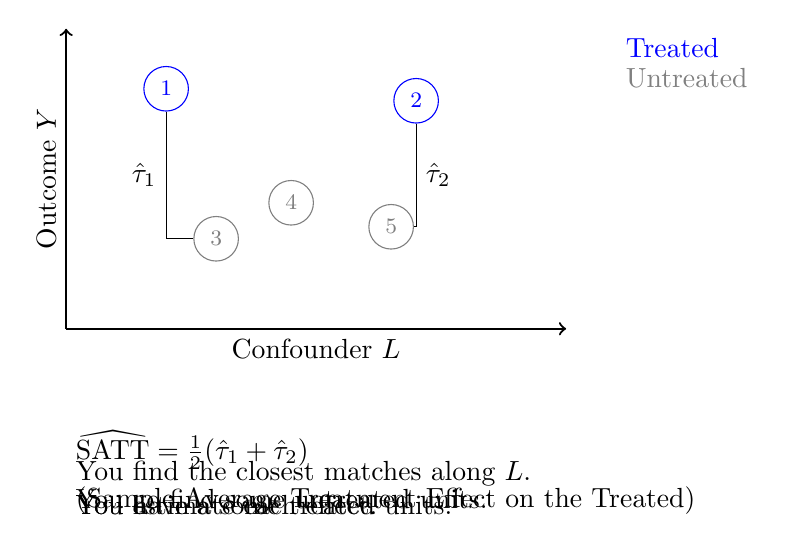
\begin{tikzpicture}[x = 2.5in, y = 1.5in]
\node at (0,-.3) {};
\draw[->, thick] (0,0) -- node[midway, below] {Confounder $L$} (1,0);
\draw[->, thick] (0,0) -- node[midway, above, rotate = 90] {Outcome $Y$} (0,1);
\node[anchor = north west, blue] at (1.1,1) {Treated};
\node[blue, draw, circle, font = \footnotesize] (p1) at (.2,.8) {$1$};
\node[blue, draw, circle, font = \footnotesize] (p2) at (.7,.76) {$2$};
\onslide<2->{
\node[anchor = north west, gray] at (1.1,.9) {Untreated};
\node[gray, draw, circle, font = \footnotesize] (p3) at (.3,.3) {$3$};
\node[gray, draw, circle, font = \footnotesize] (p4) at (.45,.42) {$4$};
\node[gray, draw, circle, font = \footnotesize] (p5) at (.65,.34) {$5$};
}
\draw<4-> (p3) -| node[pos = .75, left] {$\hat\tau_1$} (p1);
\draw<5-> (p5) -| node[pos = .75, right] {$\hat\tau_2$} (p2);
\node<6->[anchor = south west] at (0,-.5) {$\widehat{\text{SATT}} = \frac{1}{2}(\hat\tau_1 + \hat\tau_2)$};
\node<1>[anchor = south west] at (0,-.65) {You have a some treated units.};
\node<2>[anchor = south west] at (0,-.65) {You go find some untreated units.};
\node<3-5>[anchor = south west, align = left] at (0,-.65) {You find the closest matches along $L$.\\You estimate each effect.};
\node<6>[anchor = south west] at (0,-.65) {(Sample Average Treatment Effect on the Treated)};
\end{tikzpicture}
\end{frame}

\begin{frame}{Why matching is great} \pause

\begin{enumerate}[<+->]
\item Completely transparent that $Y_i^1$ is observed
\item Completely transparent how we estimate $\hat{Y}_i^0$\\(from the matched unit)
\item Easy to explain
\begin{itemize}
\item We had some treated units
\item We found comparable control units
\item We took a mean difference
\end{itemize}
\item Can assess quality of matches before we look at the outcome
\item Model-free${}^*$
\begin{itemize}
\item ${}^*$ but you have to define what makes a match ``good''
\end{itemize}
\end{enumerate}

\end{frame}

\begin{frame}{Matching: A word of warning\footnote{Sekhon, J. S. (2009). \bref{http://sekhon.berkeley.edu/papers/annualreview.pdf}{Opiates for the matches: Matching methods for causal inference.} Annual Review of Political Science, 12(1), 487-508.}} \pause

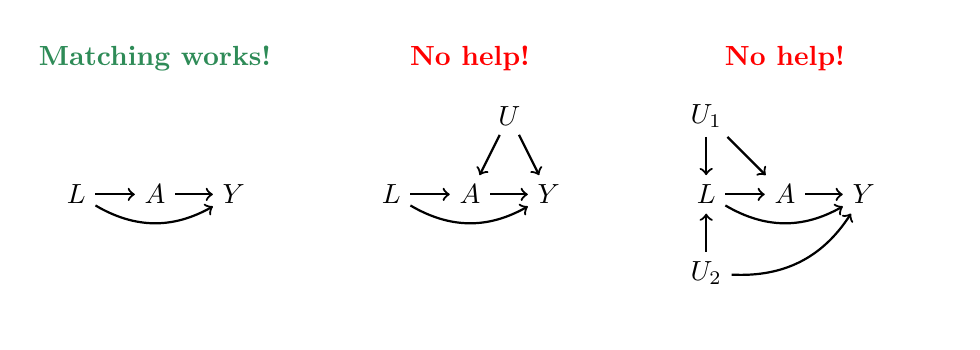
\begin{tikzpicture}
\node at (11,-1.5) {};
\node at (-.5,2) {};
\node (l) at (0,0) {$L$};
\node (a) at (1,0) {$A$};
\node (y) at (2,0) {$Y$};
\draw[->, thick] (l) -- (a);
\draw[->, thick] (l) to[bend right] (y);
\draw[->, thick] (a) -- (y); \pause
\node[anchor = north, seagreen, font = \bf] at (1,2) {Matching works!}; \pause
\node[anchor = north, red, font = \bf] at (5,2) {No help!};
\node (l) at (4,0) {$L$};
\node (a) at (5,0) {$A$};
\node (u) at (5.5,1) {$U$};
\node (y) at (6,0) {$Y$};
\draw[->, thick] (l) -- (a);
\draw[->, thick] (l) to[bend right] (y);
\draw[->, thick] (a) -- (y);
\draw[->, thick] (u) -- (a);
\draw[->, thick] (u) -- (y); \pause
\node[anchor = north, red, font = \bf] at (9,2) {No help!};
\node (l) at (8,0) {$L$};
\node (a) at (9,0) {$A$};
\node (u1) at (8,1) {$U_1$};
\node (u2) at (8,-1) {$U_2$};
\node (y) at (10,0) {$Y$};
\draw[->, thick] (l) -- (a);
\draw[->, thick] (l) to[bend right] (y);
\draw[->, thick] (a) -- (y);
\draw[->, thick] (u1) -- (a);
\draw[->, thick] (u1) -- (l);
\draw[->, thick] (u2) -- (l);
\draw[->, thick] (u2) to[bend right] (y);
\end{tikzpicture}
\onslide<6->{Matching is an estimation strategy.} \\
\onslide<7->{It does not solve identification problems.}\\
\onslide<8->{Matching is only as good as your DAG!}

\end{frame}

\subsection{Matching in univariate settings: Algorithms}

\tcframe

\begin{frame}{Matching in univariate settings: Algorithms}

\begin{itemize}
\item Caliper or no caliper
\item 1:1 vs $k$:1
\item With replacement vs without replacement
\item Greedy vs optimal
\end{itemize}

\end{frame}

\begin{frame}{Caliper or no caliper matching}

\centering
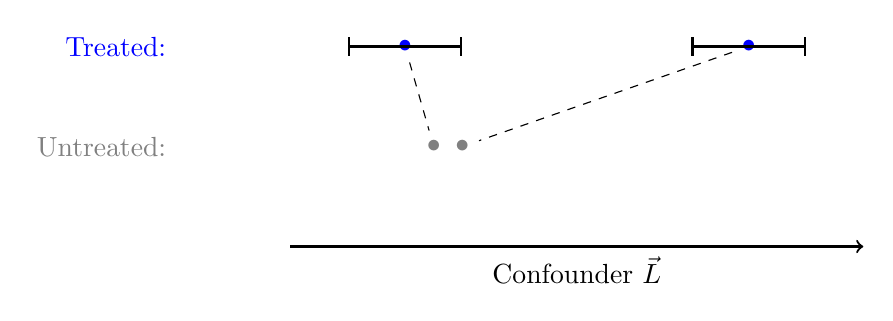
\begin{tikzpicture}[x = .6\textwidth, y = .5in]
\node[anchor = east, blue] at (-.2,1) {Treated:};
\node[anchor = east, gray] at (-.2,0) {Untreated:};
\node[blue] (p1) at (.2,1) {$\bullet$};
\node[gray] (p3) at (.25,0) {$\bullet$};
\onslide<1-5>{
\node[blue] (p2) at (.8,1) {$\bullet$};
\node[gray] (p4) at (.3,0) {$\bullet$};
}
\onslide<6->{
\node[blue, opacity = .1] (p2) at (.8,1) {$\bullet$};
\node[gray, opacity = .1] (p4) at (.3,0) {$\bullet$};
}
\draw[->, thick] (0,-1) -- node[midway, below] {Confounder $\vec{L}$} (1,-1);
\draw<2->[dashed] (p1) -- (p3);
\draw<3-5>[dashed] (p2) -- (p4);
\draw<6->[dashed, opacity = .1] (p2) -- (p4);
\draw<4->[|-|, thick] (.1,1) -- (.3,1);
\draw<4-5>[|-|, thick] (.7,1) -- (.9,1);
\draw<6->[|-|, thick, opacity = .1] (.7,1) -- (.9,1);
\end{tikzpicture}
\onslide<5->{
\begin{itemize}
\item Caliper: A radius around a treated unit such that we would rather drop the unit than make a match beyond that radius
\onslide<7->{
\item Feasible Sample Average Treatment Effect on the Treated (FSATT): Average among treated units for whom an acceptable match exists
}
\end{itemize}
}
\end{frame}

\begin{frame}{1:1 vs $k$:1 matching}

\centering
\begin{tikzpicture}[x = .6\textwidth, y = .5in]
\node[anchor = east, blue] at (-.2,1) {Treated:};
\node[anchor = east, gray] at (-.2,0) {Untreated:};
\node[blue] (p1) at (.2,1) {$\bullet$};
\node[gray] (p2) at (.25,0) {$\bullet$};
\node[gray] (p3) at (.3,0) {$\bullet$};
\node[blue] (p4) at (.8,1) {$\bullet$};
\node[gray] (p5) at (.76,0) {$\bullet$};
\node[gray] (p6) at (.81,0) {$\bullet$};
\draw[->, thick] (0,-1) -- node[midway, below] {Confounder $\vec{L}$} (1,-1);
\draw<2->[dashed] (p1) -- (p2);
\draw<2->[dashed] (p4) -- (p6);
\draw<3->[dashed] (p1) -- (p3);
\draw<3->[dashed] (p4) -- (p5);
\end{tikzpicture}
\onslide<4->{
\begin{itemize}
\item Benefit of 2:1 matching
\onslide<5->{
\begin{itemize}
\item Lower variance. Averaging over more cases.
\end{itemize}
}
\item Benefit of 1:1 matching
\onslide<6->{
\begin{itemize}
\item Lower bias. Only the best matches.
\end{itemize}
}
\onslide<7->{
\item Greater $k \rightarrow$ lower variance, higher bias
}
\end{itemize}
}
\end{frame}

\begin{frame}{With replacement vs without replacement matching}

\centering
\begin{tikzpicture}[x = .6\textwidth, y = .5in]
\node[anchor = east, blue] at (-.2,1) {Treated:};
\node[anchor = east, gray] at (-.2,0) {Untreated:};
\node[blue] (p1) at (.2,1) {$\bullet$};
\node[gray] (p2) at (.25,0) {$\bullet$};
\node[blue] (p3) at (.3,1) {$\bullet$};
\node[gray] (p4) at (.8,0) {$\bullet$};
\draw[->, thick] (0,-1) -- node[midway, below] {Confounder $\vec{L}$} (1,-1);
\draw<2->[dashed] (p1) -- (p2);
\draw<3->[dashed] (p3) -- node[midway, above] {?} (p4);
\draw<4->[dashed] (p3) -- node[midway, right] {?} (p2);
\end{tikzpicture}
\onslide<4->{
\begin{itemize}
\item Benefit of matching without replacement
\onslide<5->{
\begin{itemize}
\item Lower variance. Averaging over more cases.
\end{itemize}
}
\item Benefit of matching with replacement
\onslide<6->{
\begin{itemize}
\item Lower bias. Better matches.
\end{itemize}
}
\end{itemize}
}
\end{frame}

\begin{frame}{Greedy vs optimal matching\footnote{Gu, X. S., \& Rosenbaum, P. R. (1993). \bref{https://www.tandfonline.com/doi/abs/10.1080/10618600.1993.10474623}{Comparison of multivariate matching methods: Structures, distances, and algorithms.} Journal of Computational and Graphical Statistics, 2(4), 405-420.}}

\centering
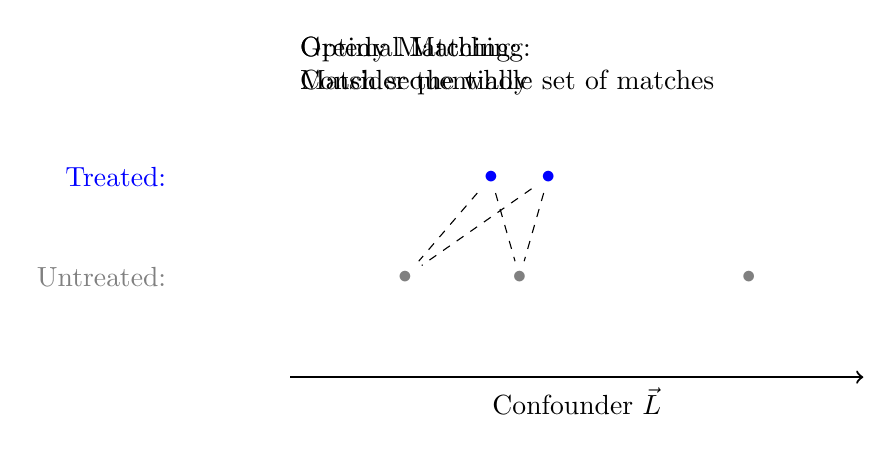
\begin{tikzpicture}[x = .6\textwidth, y = .5in]
\node[anchor = north west, align = left] at (0,2.5) {};
\node[anchor = east, blue] at (-.2,1) {Treated:};
\node[anchor = east, gray] at (-.2,0) {Untreated:};
\node[blue] (p1) at (.35,1) {$\bullet$};
\node[gray] (p2) at (.4,0) {$\bullet$};
\node[blue] (p3) at (.45,1) {$\bullet$};
\node[gray] (p4) at (.2,0) {$\bullet$};
\node[gray] (p5) at (.8,0) {$\bullet$};
\draw[->, thick] (0,-1) -- node[midway, below] {Confounder $\vec{L}$} (1,-1);
\node<2-4>[anchor = north west, align = left] at (0,2.5) {Greedy Matching:\\Match sequentially};
\draw<3-4>[dashed] (p1) -- (p2);
\draw<4-4>[dashed] (p3) -- (p4);
\node<5->[anchor = north west, align = left] at (0,2.5) {Optimal Matching:\\Consider the whole set of matches};
\draw<5->[dashed] (p1) -- (p4);
\draw<5->[dashed] (p3) -- (p2);
\end{tikzpicture}
\onslide<6->{
\begin{itemize}
\item Optimal is better. Just computationally harder.
\end{itemize}
}
\end{frame}

\begin{frame}{Matching in univariate settings: Algorithms (recap)}

\begin{itemize}
\item Caliper or no caliper
\item 1:1 vs $k$:1
\item With replacement vs without replacement
\item Greedy vs optimal
\end{itemize}

\end{frame}

\subsection{Matching in multivariate settings: Distance metrics}

\tcframe

\begin{frame}{What if $\vec{L}$ is multivariate?}

\centering
\scalebox{.8}{
\begin{tikzpicture}
\node at (-2.5,-1.5) {};
\node at (6.5,5.5) {};
\onslide<2->{
\draw[->, thick] (-2,-1) -- node[midway, below] {$L_1$} (7,-1);
\draw[->, thick] (-2,-1) -- node[midway, left] {$L_2$} (-2,5);
}
\onslide<5->{
\draw[thick, dashed] (0,0) -- node[midway, left, font = \small] {Length = 4} (0,4);
\draw[thick, dashed] (0,4) -- node[midway, above, font = \small] {Length = 3} (3,4);
}
\onslide<6->{
\draw[thick, dashed] (0,0) -- node[midway, right, font = \small] {Length = 5} (3,4);
}
\onslide<7->{
\draw[thick, dashed] (0,0) -- node[midway, below, font = \small] {Length = 6} (6,0);
}
\onslide<3->{
\node[blue] (treated) at (0,0) {$\bullet$};
\node[gray] (a) at (3,4) {$\bullet$};
\node[gray] (b) at (6,0) {$\bullet$};
\node[anchor = north east, font = \small, blue] at (treated) {Treated};
\node[anchor = south west, font = \small, gray] at (a) {Untreated 1};
\node[anchor = south west, font = \small, gray] at (b) {Untreated 2};
}
\end{tikzpicture}
} \vskip .1in

\onslide<4->{Which untreated unit should be the match?}

\end{frame}

\begin{frame}{What if $\vec{L}$ is multivariate? We need a \bblue{distance metric}}

\centering
\scalebox{.4}{
\begin{tikzpicture}
\node at (-2.5,-1.5) {};
\node at (6.5,5.5) {};
\draw[->, thick] (-2,-1) -- node[midway, below] {$L_1$} (7,-1);
\draw[->, thick] (-2,-1) -- node[midway, left] {$L_2$} (-2,5);
\draw[thick, dashed] (0,0) -- node[midway, left, font = \small] {Length = 4} (0,4);
\draw[thick, dashed] (0,4) -- node[midway, above, font = \small] {Length = 3} (3,4);
\draw[thick, dashed] (0,0) -- node[midway, right, font = \small] {Length = 5} (3,4);
\draw[thick, dashed] (0,0) -- node[midway, below, font = \small] {Length = 6} (6,0);
\node[blue] (treated) at (0,0) {$\bullet$};
\node[gray] (a) at (3,4) {$\bullet$};
\node[gray] (b) at (6,0) {$\bullet$};
\node[anchor = north east, font = \small, blue] at (treated) {Treated};
\node[anchor = south west, font = \small, gray] at (a) {Untreated 1};
\node[anchor = south west, font = \small, gray] at (b) {Untreated 2};
\end{tikzpicture}
}
\onslide<2->{
\begin{itemize}
\item Manhattan distance:\onslide<3->{ $d(i,j) = \sum_p \lvert L_{pi} - L_{pj}\rvert $}
\onslide<4->{
\begin{itemize}
\item $d(\text{Treated, Untreated 1}) = 3 + 4 = 7$
\item $d(\text{Treated, Untreated 2}) = 6 + 0 = 6$ $\checkmark$
\end{itemize}
}
\item Euclidean distance: \onslide<5->{$d(i,j) = \sqrt{\sum_p \left( L_{pi} - L_{pj}\right)^2} $}
\onslide<6->{
\begin{itemize}
\item $d(\text{Treated, Untreated 1}) = \sqrt{3^2 + 4^2} = 5$ $\checkmark$
\item $d(\text{Treated, Untreated 2}) = \sqrt{6^2 + 0^2} = 6$
\end{itemize}
\onslide<7->{\item It depends on the distance metric!}
\end{itemize}
}
}

\end{frame}

\begin{frame}{A common distance metric: Mahalanobis distance}
\pause
Motivated by two principles \pause
\begin{itemize}[<+->]
\item Principle 1: Address unequal variances
\begin{itemize}
\item Suppose $L_1$ ranges uniformly from 0 to 100
\item Suppose $L_2$ ranges uniformly from 0 to 1
\item We might correct for this so $L_1$ doesn't dominate the distance
\end{itemize}
\item Principle 2: Address correlations
\begin{itemize}
\item Suppose $L_1$ and $L_2$ are very correlated
\item Suppose $L_3$ is independent
\item We should care about a correlation-corrected distance
\end{itemize}
\end{itemize} \pause \vskip .1in
$$d(i,j) = \sqrt{\left(\vec{L}_i - \vec{L}_j\right)^T\Sigma^{-1}\left(\vec{L}_i - \vec{L}_j\right)}$$
where $\Sigma = \V(\vec{L})$, the variance-covariance matrix
\end{frame}

\begin{frame}{A common distance metric: Exact matching}
\pause

\begin{itemize}
\item Equivalent to nonparametric stratification \pause
\item Infinite distance if any confounder is different!
\end{itemize} \vskip .1in
$$
d(i,j) = \begin{cases}
0 &\text{if }\vec{L}_i = \vec{L}_j \\
\infty &\text{if }\vec{L}_i \neq \vec{L}_j \\
\end{cases}
$$
Often leads to \bblue{no matches at all}
\end{frame}

\begin{frame}{A common distance metric: Coarsened exact matching\footnote{Iacus, S. M., King, G., \& Porro, G. (2012). \bref{https://www.cambridge.org/core/journals/political-analysis/article/causal-inference-without-balance-checking-coarsened-exact-matching/5ABCF5B3FC3089A87FD59CECBB3465C0}{Causal inference without balance checking: Coarsened exact matching.} Political Analysis, 20(1), 1-24.}}

\pause
\begin{itemize}
\item Define $\tilde{\vec{L}}$ to be a coarsened version of $\vec{L}$ \pause
\begin{itemize}
\item Example: Convert all continuous values to decile categories
\end{itemize} \pause
\item Match exactly on $\tilde{\vec{L}}$
\end{itemize} \pause \vskip .1in
$$
d(i,j) = \begin{cases}
0 &\text{if }\tilde{\vec{L}}_i = \tilde{\vec{L}}_j \\
\infty &\text{if }\tilde{\vec{L}}_i \neq \tilde{\vec{L}}_j \\
\end{cases}
$$
\begin{itemize} \pause
\item Benefit: Very transparent \pause
\item Drawback: Ignores $\vec{L}$ within $\tilde{\vec{L}}$ \pause
\item Best used as preprocessing for regression \pause
\begin{itemize}
\item Conduct coarsened exact matching \pause
\item Conduct regression on the matched dataset \pause
\item See paper
\end{itemize}
\end{itemize}
\end{frame}

\begin{frame}{A common distance metric: Propensity scores}

\centering
\scalebox{.6}{
\begin{tikzpicture}
\node at (-2.5,-1.5) {};
\node at (6.5,5.5) {};
\draw[->, thick] (-2,-1) -- node[midway, below] {$L_1$} (7,-1);
\draw[->, thick] (-2,-1) -- node[midway, left] {$L_2$} (-2,5);
\draw[thick, dashed] (0,0) -- node[midway, left, font = \small] {Length = 4} (0,4);
\draw[thick, dashed] (0,4) -- node[midway, above, font = \small] {Length = 3} (3,4);
\draw[thick, dashed] (0,0) -- node[midway, right, font = \small] {Length = 5} (3,4);
\draw[thick, dashed] (0,0) -- node[midway, below, font = \small] {Length = 6} (6,0);
\node[blue] (treated) at (0,0) {$\bullet$};
\node[gray] (a) at (3,4) {$\bullet$};
\node[gray] (b) at (6,0) {$\bullet$};
\node[anchor = north east, font = \small, blue] at (treated) {Treated};
\node[anchor = south west, font = \small, gray] at (a) {Untreated 1};
\node[anchor = south west, font = \small, gray] at (b) {Untreated 2};
\end{tikzpicture}
} \vskip .2in \pause
Now suppose only $L_2$ is related to treatment. $L_1$ doesn't matter.\\
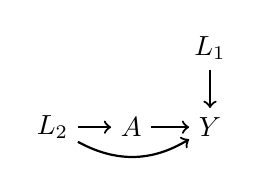
\begin{tikzpicture}
\node (l2) at (0,0) {$L_2$};
\node (l1) at (2,1) {$L_1$};
\node (a) at (1,0) {$A$};
\node (y) at (2,0) {$Y$};
\draw[->, thick] (l2) -- (a);
\draw[->, thick] (l2) to[bend right] (y);
\draw[->, thick] (l1) -- (y);
\draw[->, thick] (a) -- (y);
\end{tikzpicture}\\ \pause
Which match do you pick? \pause Untreated 2! Perfect match.

\end{frame}

\begin{frame}{A common distance metric: Propensity scores}
Propensity score: $\pi_i = \P(A = 1\mid \vec{L} = \vec\ell_i)$ \pause
\begin{itemize}
\item Univariate summary of all confounders \pause
\item In expectation, a sample balanced on $\pi$ is balanced on $\vec{L}$
\begin{itemize}
\item Rosenbaum \& Rubin theorem\footnote{Rosenbaum, P. R., \& Rubin, D. B. (1983). \bref{https://doi.org/10.1093/biomet/70.1.41}{The central role of the propensity score in observational studies for causal effects.} Biometrika, 70(1), 41-55.}
\end{itemize}
\end{itemize}
\end{frame}

\begin{frame}{A common distance metric: Propensity scores}

Propensity scores can be nonparametric or parametric.
\begin{itemize} \pause
\item Nonparametric: $\hat\pi_i$ is the proportion treated in the sample stratum $\vec{L} = \vec\ell_i$. \pause
\item Parametric: Often estimated as
\begin{itemize}
\item Fit logistic regression
$$\text{logit}\left(\P(A = 1\mid \vec{L})\right) = \alpha + \vec{L}\vec\beta$$ \pause
\item Predict the probability of treatment
$$\hat\pi_i = \text{logit}^{-1}\left(\hat\alpha + \vec\ell_i\hat{\vec\beta}\right)$$ \vspace{-.2in}
\end{itemize}
\end{itemize} \pause
Propensity score distance for matching:
$$d(i,j) = \lvert \hat\pi_i - \hat\pi_j\rvert $$

\end{frame}

\begin{frame}{Why propensity scores are nice} \pause

\begin{itemize}
\item Multivariate $\vec{L}_i$ to univariate $\pi_i$ \pause
\begin{itemize}
\item Easy to reason about \pause
\item Can directly visualize the univariate matches
\end{itemize} \pause
\item Mathematical guarantees in expectation \pause
\item Intuitive: Prioritizes covariates that predict treatment
\end{itemize}

\end{frame}

\begin{frame}{Propensity score problems: King \& Nielsen\footnote{King, G., \& Nielsen, R. (2019). \bref{https://www.cambridge.org/core/journals/political-analysis/article/whypropensity-scoresshould-not-be-usedformatching/94DDE7ED8E2A796B693096EB714BE68B}{Why propensity scores should not be used for matching.} Political Analysis, 27(4), 435-454.}}
\pause
Motivated by two designs for randomized experiments \pause
\begin{itemize}
\item Experimental ideal 1: Fully blocked \pause
\begin{itemize}
\item First, stratify units on $\vec{L}$ \pause
\item Then, randomize $A$ within blocks by a coin flip \pause
\item Imbalance on $\vec{L}$ is zero in every sample \pause
\end{itemize}
\item Experimental ideal 2: Completely randomized experiment \pause
\begin{itemize}
\item Assign each unit a known $\pi_i = \P(A = 1\mid \vec{L} = \vec\ell_i)$ \pause
\item Randomize treatment weighted by $\pi_i$ \pause
\item Imbalance on $\vec{L}$ is zero in expectation,\\but not in any particular sample \pause
\end{itemize}
\end{itemize}
In a randomized experiment, we would always choose (1). \pause \vskip .1in
But propensity score matching approximates (2). \pause \vskip .1in
King \& Nielsen claim: Better to match on $\vec{L}$ directly

\end{frame}

\begin{frame}{Propensity scores: My view}

\pause
There is no uniformly superior method. Always application-specific. \pause
\begin{itemize}
\item Propensity scores are most popular \pause
\item Other matching distances might be better in finite samples
\end{itemize} \pause \vskip .2in
Why might you use propensity scores? \pause
\begin{itemize}
\item Sometimes they are substantively meaningful\footnote{Brand, J. E., \& Xie, Y. (2010). \bref{https://journals.sagepub.com/doi/abs/10.1177/0081175012452652?casa_token=ha2yY6MUh_wAAAAA:J3P4nV3zTehU1ZMpAf-8vcPoJAMTh8m-7uM8FI-TC2hU5JSMr6C5mMcb76WMrZ4VVNfD-UmCagwZ}{Who benefits most from college? Evidence for negative selection in heterogeneous economic returns to higher education.} American Sociological Review, 75(2), 273-302.} \pause
\item Useful in other ways (e.g., weighting)
\end{itemize}

\end{frame}

\begin{frame}{Multivariate distances: Recap}

When matching on multivariate $\vec{L}$, you have to define the distance between each pair of confounder values $\vec\ell$ and $\vec\ell'$
\begin{itemize}
\item Manhattan distance
\item Euclidean distanace
\item Mahalanobis distance
\item Exact distance
\item Coarsened exact distance
\item Propensity score distance
\end{itemize}
There is no right answer! Depends on the setting.

\end{frame}

\subsection{After matching: Evaluate matched sets}

\tcframe

\begin{frame}{Evaluate the matched sets}
Why we match: So $\vec{L}$ follows a similar distribution
\begin{itemize}
\item in the treated sample
\item in the untreated sample
\end{itemize}
Whatever method, you should check that.
\begin{itemize}
\item Compare means of $\vec{L}$ across groups
\item Possibly compare interactive cells
\item Ideally, before looking at $Y$!
\end{itemize}
\end{frame}

\goalsframe

\begin{frame}{Let me know what you are thinking}

\begin{huge} \bref{https://tinyurl.com/CausalQuestions}{tinyurl.com/CausalQuestions} \end{huge}
\vskip .7in

Office hours TTh 11am-12pm and at \bref{https://calendly.com/ianlundberg/office-hours}{calendly.com/ianlundberg/office-hours}\\Come say hi!

\end{frame}

\end{document}

